\section{Справочные сведения о походе} 

\subsection{Общие сведения о походе}

\begin{table}[h]
	\centering
	\begin{tabular}{|l|l|}
		\hline
		Проводящая организация & Горная Секция МФТИ г. Долгопрудный, Московская обл. \\
		\hline
		Маршрутная книжка & №3/26, выдана МКК ФСТ г. Королёв Московской области \\
		\hline
		Район похода & Южный Урал, Национальный парк «Таганай» \\
		\hline
		Вид туризма & Лыжный \\
		\hline
		Категория сложности похода & Первая \\
		\hline
		Сроки проведения похода & С 04 по 09 января 2026~г. \\
		\hline
		Продолжительность маршрута & 6 дней\\
		\hline
		Протяжённость маршрута & всего: 87.4 км \newline в зачёт: 82.2 км \\
		\hline
		Суммарный перепад высот &2400~м \\
		\hline
		Эквивалентная протяжённость & \alert{128,8 км} \\
		\hline
	\end{tabular}
\end{table}

\clearpage

\subsection{Список участников}
\vspace{-0.4cm}

\begin{table}[h!]
	\centering
	\resizebox{0.87\textwidth}{!}{%
		\begin{tabular}{|>{\centering\arraybackslash}m{0.015\linewidth}|>{\centering\arraybackslash}m{0.17\linewidth}|>{\centering\arraybackslash}m{0.22\linewidth}|>{\centering\arraybackslash}m{0.05\linewidth}|>{\centering\arraybackslash}m{0.15\linewidth}|>{\centering\arraybackslash}m{0.180\linewidth}|}
			\hline
			\textbf{№} &
			\textbf{Фото} &
			\textbf{ФИО} &
			\textbf{г.р.} &
			\textbf{Обязанности в группе} &
			\textbf{Туристский опыт} \\
			\hline			
			
			1	&	\includegraphics[width=0.99\linewidth]{pics/portraits/as.jpg}	& Смирнов Александр Сергеевич	&	2004	&	Руководитель	& 3ГУ, 2ЛУ \\
			\hline
			2	& \includegraphics[width=0.99\linewidth]{pics/portraits/ab.jpg}	& Бернакевич Анна Сергеевна	&	2003	&	Участник	&  \\
			\hline
			3	&	\includegraphics[width=0.99\linewidth]{pics/portraits/pk.jpg}	&	Косарев Павел Алексеевич	&	2006	&	Финансист	&	1ГУ, 1ПУ \\
			\hline
			4	&	\includegraphics[width=0.99\linewidth]{pics/portraits/ao.jpg}	&	Остапив Алексей Юрьевич	&	1998	&	Логист	&	2ГУ, 1ГР, 1ПР \\
			\hline
			5	&	\includegraphics[width=0.99\linewidth]{pics/portraits/kr.jpg}	&	Рябкова Камилла Александровна	&	2003	&	Снаряженец	&	1ГУ, 2ЛУ \\
			\hline
			6	&	\includegraphics[width=0.99\linewidth]{pics/portraits/mc.jpg}	&	Чернецкий Михаил Георгиевич	&	1963	&	Реммастер	&	5ГУ, 2ГР, 2ЛУ \\
			\hline
			7	&	\includegraphics[width=0.99\linewidth]{pics/portraits/ms.jpg}	&	Сулимов Марк Дмитриевич	&	2004	&	Хронометрист	&	 \\
			\hline
			8	&	\includegraphics[width=0.99\linewidth]{pics/portraits/dh.jpg}	&	Харитонов Даниил Николаевич	&	2005	&	Хронометрист	&	 \\
			\hline
			9	&	\includegraphics[width=0.99\linewidth]{pics/portraits/ayu.jpg}	&	Юшин Александр Евгеньевич	&	2004	&	Медик	&	 \\
			\hline
		\end{tabular}%
	}
\end{table}

\clearpage


\subsection{Подробная нитка маршрута}
\textbf{Заявленная:} кур. Джилысу~--- ФГС~--- д.р. Чон-Кызыл-Суу~--- д.р. Саватор~---  \textbf{пер. Саватор~(1А, 4000)}~--- д.р. Киче-Кызыл-Суу~---  \textbf{пер.~Перемётный (1А, 4026)}~--- д.р. Джукучак~--- \textbf{пер.~Ашутор Западный (1А, 3700)}~--- д.р. Ашукашкасуу~---  д.р. Джууку~---  д.р. Иттиши~---  \textbf{пер. Иттиш ~(1А, 3895)}~---  д.р. Ит-Тиши (юж.)~---   д.р. Кашкасу~---   озёра Кашкасу~---  в. Марс (н/к, 4345)~---  \textbf{пер.~Кашкасу  (1А, 3890)}~--- д.р. Ашукашкасуу~--- д.р. Джууку~--- слияние р. Джууку и Джукучак.

\textbf{Пройденная:} ух бля


\textbf{Причины изменения нитки маршрута:} ну как бы вам помягче то сказать

\clearpage

\subsection{Схема маршрута}

\begin{figure}[h!tbp]
	\centering
	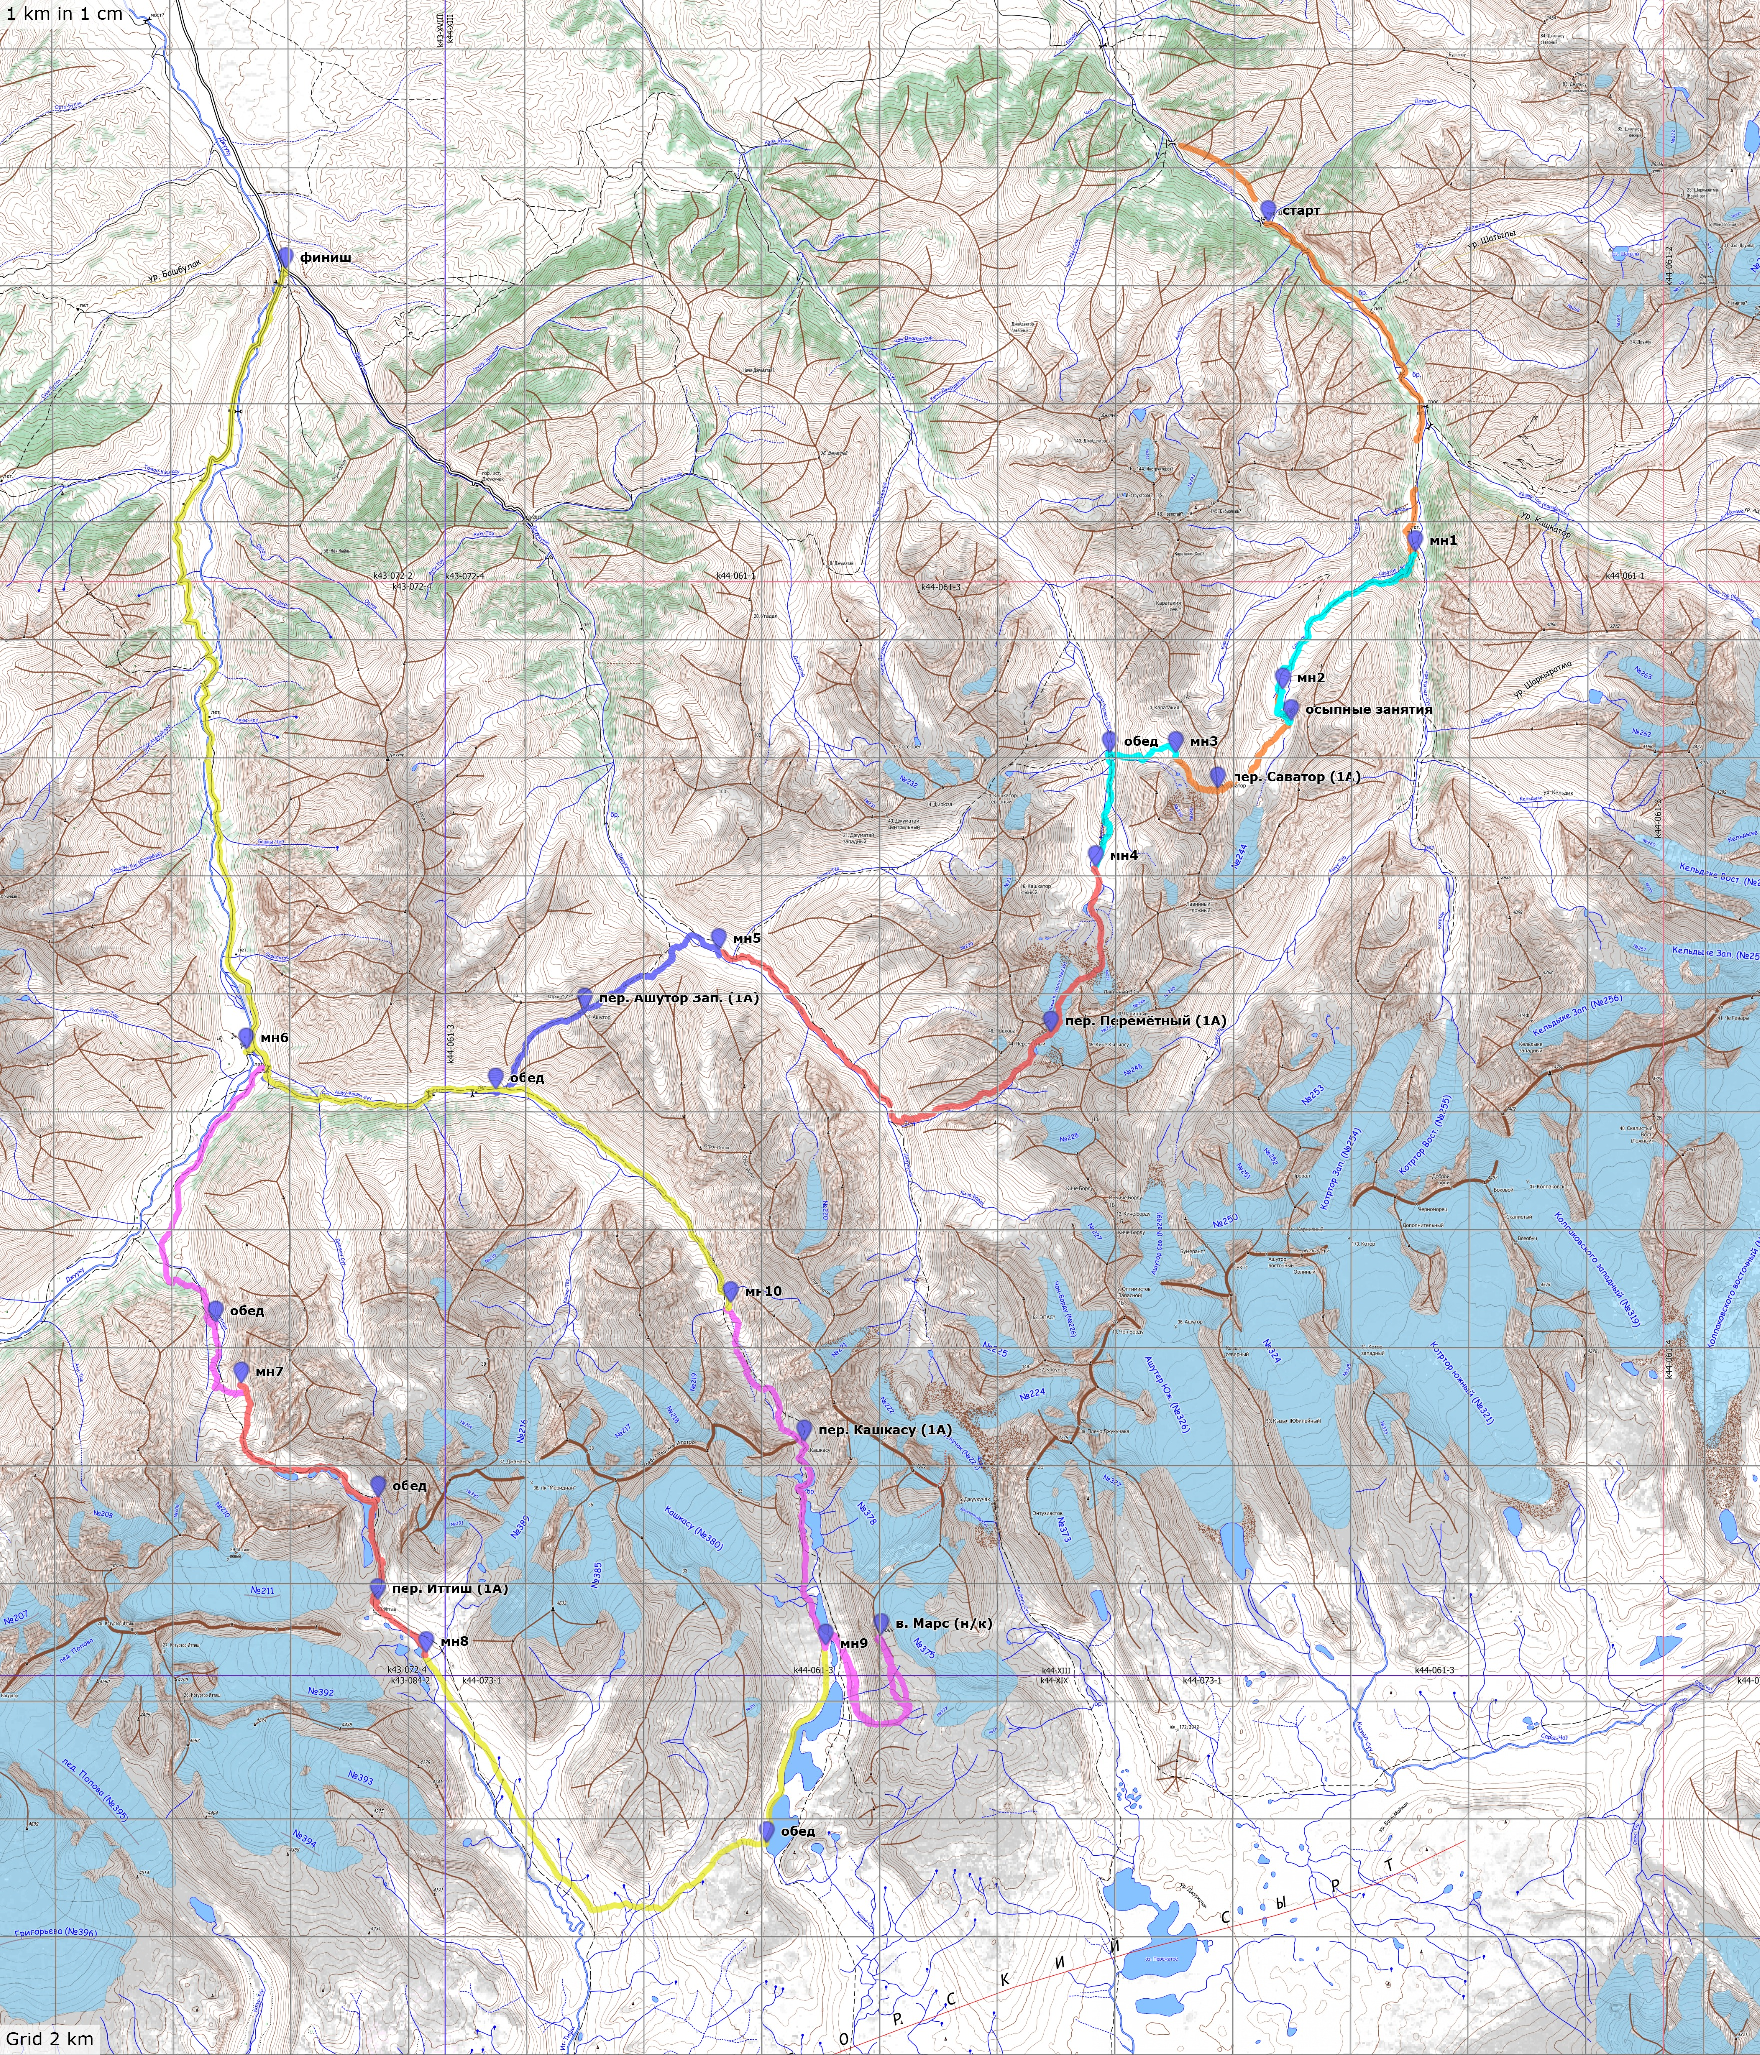
\includegraphics[width=0.99\linewidth]{pics/maps/map}
	\caption{Обзорная схема маршрута}
\end{figure}

\clearpage

\subsection{Высотный профиль маршрута}

\begin{figure}[h!]
	\centering
	\includegraphics[width=0.92\linewidth]{pics/elevation_vs_time}
	\includegraphics[width=0.92\linewidth]{pics/elevation_vs_distance}
	\caption{Высотный профиль маршрута, расстояние дано с $k=1.2$}
	\label{fig:heights}
\end{figure}

\clearpage

\subsection{Определяющие препятствия маршрута}

\begin{table}[h!]
		\begin{tabular}{|>{\centering\arraybackslash}m{0.16\linewidth}|>{\centering\arraybackslash}m{0.03\linewidth}|>{\centering\arraybackslash}m{0.45\linewidth}|>{\centering\arraybackslash}m{0.25\linewidth}|}
			\hline
			\textbf{Вид препятствия, высота} &
			\begin{turn}{90}\textbf{к. тр.}\end{turn} &
			\textbf{Характеристика препятствия} &
			\textbf{Способ прохождения} \\
			\hline			
			в. Двуглавая Сопка (Перья) (1009) & н/к &  Набор высоты~--- 350~м на 900~м. От приюта <<Белый ключ>> по оборудованным лестницам, далее~--- по склону крутизной до 25\degree. Движение осложнено тем, что склон раскатан посетителями & Пешком\\
			\hline			
			в. Круглица	 (1178)  & н/к & Набор высоты от пер. Долина Сказок (Таганайская долина)~--- 168 м на 1 км. Крутизна
			склона~---  до 15\degree. В начале склона лес, выше~---  курумник
			г. и мелкие скалы & До перевала Долина Сказок~--- на лыжах, далее до вершины по курумнику~--- пешком \\
			\hline
			в. Дальний Таганай (1112)  & н/к & Набор
			высоты 370 м на 2.5 км. Крутизна
			склона до 15--20\degree. Тропа, ГТЛ=10 см, последние
			200 м~--- участок открытой тундры с
			наледями и частично обнаженным
			грунтом & Пешком\\
			\hline
			в. Ицыл (1049)  & 1А & Набор высоты 215~м на 2 км. Крутизна склона до 10--15°.
			Часть склона~--- лесистая, часть~--- россыпи курумника, мелкие
			скалы & На лыжах, затем пешком по границе зон леса и курумника на хребет, затем по хребту пешком
			до вершины. Спуск с вершины до седловины пешком, далее на восток на лыжах\\
			\hline
			в. Крутой Ключ (782)  & н/к & От седловины движение по скальному гребню 200 м без набора высоты до лесной площадки, затем подъём на скальные
			выходы с курумником. Набор высоты~--- 50~м на 400~м.
			Крутизна склона 15--25\degree & Пешком, самостраховка лыжными/треккинговыми палками\\

			\hline
	\end{tabular}%
\end{table}

\clearpage

\subsection{Общая характеристика района проведения похода}


\subsection{Туристские особенности района}
Район хорошо подходит для несложных лыжных походов 1 к.с. С одной стороны, здесь можно чувствовать себя в относительной безопасности: большая часть маршрута проходит по национальному парку с развитой сетью приютов, а близость цивилизации, спасательных служб и наличие связи на вершинах снижают негативные последствия от возможных ошибок для новичков. С другой стороны, маршруты здесь зрелищнее и динамичнее, чем равнинные походы в Центральной России. Горный рельеф позволяет за один переход пересечь несколько климатических зон, подняться на живописные смотровые точки и получить опыт для будущих, более сложных путешествий по пересечённой местности.
\clearpage